%% FEUP THESIS STYLE for LaTeX2e
%% how to use feupteses (English version)
%%
%% FEUP, JCL & JCF, 31 July 2012
%%
%% PLEASE send improvements to jlopes at fe.up.pt and to jcf at fe.up.pt
%%

%%========================================
%% Commands: pdflatex tese
%%           bibtex tese
%%           makeindex tese (only if creating an index) 
%%           pdflatex tese
%% Alternative:
%%          latexmk -pdf tese.tex
%%========================================

\documentclass[11pt,a4paper,twoside,openright]{report}

%% For iso-8859-1 (latin1), comment next line and uncomment the second line
\usepackage[utf8]{inputenc}
%\usepackage[latin1]{inputenc}

%% English version

%% MIEIC options
\usepackage[mieic]{feupteses}
%\usepackage[mieic,juri]{feupteses}
%\usepackage[mieic,final]{feupteses}
%\usepackage[mieic,final,onpaper]{feupteses}

%% Additional options for feupteses.sty: 
%% - onpaper: links are not shown (for paper versions)
%% - backrefs: include back references from bibliography to citation place

%% Uncomment the next lines if side by side graphics used
%\usepackage[lofdepth,lotdepth]{subfig}
%\usepackage{graphicx}
%\usepackage{float}

\usepackage{todonotes}
\setlength{\marginparwidth}{2cm}
\usepackage{amsmath}
%% Include color package
\usepackage{color}
\definecolor{cloudwhite}{cmyk}{0,0,0,0.025}

%% Include source-code listings package
\usepackage{listings}
\lstset{ %
 language=C,                        % choose the language of the code
 basicstyle=\footnotesize\ttfamily,
 keywordstyle=\bfseries,
 numbers=left,                      % where to put the line-numbers
 numberstyle=\scriptsize\texttt,    % the size of the fonts that are used for the line-numbers
 stepnumber=1,                      % the step between two line-numbers. If it's 1 each line will be numbered
 numbersep=8pt,                     % how far the line-numbers are from the code
 frame=tb,
 float=htb,
 aboveskip=8mm,
 belowskip=4mm,
 backgroundcolor=\color{cloudwhite},
 showspaces=false,                  % show spaces adding particular underscores
 showstringspaces=false,            % underline spaces within strings
 showtabs=false,                    % show tabs within strings adding particular underscores
 tabsize=2,	                    % sets default tabsize to 2 spaces
 captionpos=b,                      % sets the caption-position to bottom
 breaklines=true,                   % sets automatic line breaking
 breakatwhitespace=false,           % sets if automatic breaks should only happen at whitespace
 escapeinside={\%*}{*)},            % if you want to add a comment within your code
 morekeywords={*,var,template,new}  % if you want to add more keywords to the set
}

%% Uncomment to create an index (at the end of the document)
%\makeindex

%% Path to the figures directory
%% TIP: use folder ``figures'' to keep all your figures
\graphicspath{{figures/}}

%%----------------------------------------
%% TIP: if you want to define more macros, use an external file to keep them
%some macro definitions

% format
\newcommand{\class}[1]{{\normalfont\slshape #1\/}}

% entities
\newcommand{\Feup}{Faculdade de Engenharia da Universidade do Porto}

\newcommand{\svg}{\class{SVG}}
\newcommand{\scada}{\class{SCADA}}
\newcommand{\scadadms}{\class{SCADA/DMS}}

%%----------------------------------------

%%========================================
%% Start of document
%%========================================
\begin{document}

%%----------------------------------------
%% Information about the work
%%----------------------------------------
\title{Title of the Dissertation}
\author{Name of the Author}

%% Uncomment next line for date of submission
%\thesisdate{July 31, 2008}

%%Uncomment next line for copyright text if used
%\copyrightnotice{Name of the Author, 2008}

\supervisor{Supervisor}{Name of the Supervisor}

%% Uncomment next line if necessary
%\supervisor{Second Supervisor}{Name of the Supervisor}

%% Uncomment committee stuff in the final version if used
%\committeetext{Approved in oral examination by the committee:}
%\committeemember{Chair}{Doctor Name of the President}
%\committeemember{External Examiner}{Doctor Name of the Examiner}
%\committeemember{Supervisor}{Doctor Name of the Supervisor}
%\signature

%% Specify cover logo (in folder ``figures'')
\logo{uporto-feup.pdf}

%% Uncomment next line for additional text  below the author's name (front page)
%\additionalfronttext{Preparação da Dissertação}

%%----------------------------------------
%% Preliminary materials
%%----------------------------------------

% remove unnecssary \include{} commands
\begin{Prolog}
  \chapter*{Abstract}

Here goes the abstract written in English.

Lorem ipsum dolor sit amet, consectetuer adipiscing elit. Sed vehicula
lorem commodo dui. Fusce mollis feugiat elit. Cum sociis natoque
penatibus et magnis dis parturient montes, nascetur ridiculus
mus. Donec eu quam. Aenean consectetuer odio quis nisi. Fusce molestie
metus sed neque. Praesent nulla. Donec quis urna. Pellentesque
hendrerit vulputate nunc. Donec id eros et leo ullamcorper
placerat. Curabitur aliquam tellus et diam. 

Ut tortor. Morbi eget elit. Maecenas nec risus. Sed ultricies. Sed
scelerisque libero faucibus sem. Nullam molestie leo quis
tellus. Donec ipsum. Nulla lobortis purus pharetra turpis. Nulla
laoreet, arcu nec hendrerit vulputate, tortor elit eleifend turpis, et
aliquam leo metus in dolor. Praesent sed nulla. Mauris ac augue. Cras
ac orci. Etiam sed urna eget nulla sodales venenatis. Donec faucibus
ante eget dui. Nam magna. Suspendisse sollicitudin est et mi. 

Fusce sed ipsum vel velit imperdiet dictum. Sed nisi purus, dapibus
ut, iaculis ac, placerat id, purus. Integer aliquet elementum
libero. Phasellus facilisis leo eget elit. Nullam nisi magna, ornare
at, aliquet et, porta id, odio. Sed volutpat tellus consectetuer
ligula. Phasellus turpis augue, malesuada et, placerat fringilla,
ornare nec, eros. Class aptent taciti sociosqu ad litora torquent per
conubia nostra, per inceptos himenaeos. Vivamus ornare quam nec sem
mattis vulputate. Nullam porta, diam nec porta mollis, orci leo
condimentum sapien, quis venenatis mi dolor a metus. Nullam
mollis. Aenean metus massa, pellentesque sit amet, sagittis eget,
tincidunt in, arcu. Vestibulum porta laoreet tortor. Nullam mollis
elit nec justo. In nulla ligula, pellentesque sit amet, consequat sed,
faucibus id, velit. Fusce purus. Quisque sagittis urna at quam. Ut eu
lacus. Maecenas tortor nibh, ultricies nec, vestibulum varius, egestas
id, sapien. 

Phasellus ullamcorper justo id risus. Nunc in leo. Mauris auctor
lectus vitae est lacinia egestas. Nulla faucibus erat sit amet lectus
varius semper. Praesent ultrices vehicula orci. Nam at metus. Aenean
eget lorem nec purus feugiat molestie. Phasellus fringilla nulla ac
risus. Aliquam elementum aliquam velit. Aenean nunc odio, lobortis id,
dictum et, rutrum ac, ipsum. 

Ut tortor. Morbi eget elit. Maecenas nec risus. Sed ultricies. Sed
scelerisque libero faucibus sem. Nullam molestie leo quis
tellus. Donec ipsum. Nulla lobortis purus pharetra turpis. Nulla
laoreet, arcu nec hendrerit vulputate, tortor elit eleifend turpis, et
aliquam leo metus in dolor. Praesent sed nulla. Mauris ac augue. Cras
ac orci. Etiam sed urna eget nulla sodales venenatis. Donec faucibus
ante eget dui. Nam magna. Suspendisse sollicitudin est et mi. 

Phasellus ullamcorper justo id risus. Nunc in leo. Mauris auctor
lectus vitae est lacinia egestas. Nulla faucibus erat sit amet lectus
varius semper. Praesent ultrices vehicula orci. Nam at metus. Aenean
eget lorem nec purus feugiat molestie. Phasellus fringilla nulla ac
risus. Aliquam elementum aliquam velit. Aenean nunc odio, lobortis id,
dictum et, rutrum ac, ipsum. 

Ut tortor. Morbi eget elit. Maecenas nec risus. Sed ultricies. Sed
scelerisque libero faucibus sem. Nullam molestie leo quis
tellus. Donec ipsum. 

\chapter*{Resumo}

O Resumo fornece ao leitor um sumário do conteúdo da dissertação.
Deverá ser breve mas conter detalhe suficiente e, uma vez que é a porta
de entrada para a dissertação, deverá dar ao leitor uma boa impressão
inicial.

Este texto inicial da dissertação é escrito no fim e resume numa
página, sem referências externas, o tema e o contexto do trabalho, a
motivação e os objectivos, as metodologias e técnicas empregues, os
principais resultados alcançados e as conclusões.

Este documento ilustra o formato a usar em dissertações na \Feup.
São dados exemplos de margens, cabeçalhos, títulos, paginação, estilos
de índices, etc. 
São ainda dados exemplos de formatação de citações, figuras e tabelas,
equações, referências cruzadas, lista de referências e índices.
%Este documento não pretende exemplificar conteúdos a usar. 
É usado texto descartável, \emph{Loren Ipsum}, para preencher a
dissertação por forma a ilustrar os formatos.

Seguem-se umas notas breves mas muito importantes sobre a versão 
provisória e a versão final do documento. 
A versão provisória, depois de verificada pelo orientador e de 
corrigida em contexto pelo autor, deve ser publicada na página 
pessoal de cada estudante/dissertação, juntamente com os dois 
resumos, em português e em inglês; deve manter a marca da água, 
assim como a numeração de linhas conforme aqui se demonstra.

A versão definitiva, a produzir somente após a defesa, em versão 
impressa (dois exemplares com capas próprias FEUP) e em versão 
eletrónica (6 CDs com "rodela" própria FEUP), deve ser limpa da marca de 
água e da numeração de linhas e deve conter a identificação, na primeira 
página, dos elementos do júri respetivo. 
Deve ainda, se for o caso, ser corrigida de acordo com as instruções 
recebidas dos elementos júri.

Lorem ipsum dolor sit amet, consectetuer adipiscing elit. Sed vehicula
lorem commodo dui. Fusce mollis feugiat elit. Cum sociis natoque
penatibus et magnis dis parturient montes, nascetur ridiculus
mus. Donec eu quam. Aenean consectetuer odio quis nisi. Fusce molestie
metus sed neque. Praesent nulla. Donec quis urna. Pellentesque
hendrerit vulputate nunc. Donec id eros et leo ullamcorper
placerat. Curabitur aliquam tellus et diam. 

Ut tortor. Morbi eget elit. Maecenas nec risus. Sed ultricies. Sed
scelerisque libero faucibus sem. Nullam molestie leo quis
tellus. Donec ipsum. Nulla lobortis purus pharetra turpis. Nulla
laoreet, arcu nec hendrerit vulputate, tortor elit eleifend turpis, et
aliquam leo metus in dolor. Praesent sed nulla. Mauris ac augue. Cras
ac orci. Etiam sed urna eget nulla sodales venenatis. Donec faucibus
ante eget dui. Nam magna. Suspendisse sollicitudin est et mi. 

Phasellus ullamcorper justo id risus. Nunc in leo. Mauris auctor
lectus vitae est lacinia egestas. Nulla faucibus erat sit amet lectus
varius semper. Praesent ultrices vehicula orci. Nam at metus. Aenean
eget lorem nec purus feugiat molestie. Phasellus fringilla nulla ac
risus. Aliquam elementum aliquam velit. Aenean nunc odio, lobortis id,
dictum et, rutrum ac, ipsum. 

Ut tortor. Morbi eget elit. Maecenas nec risus. Sed ultricies. Sed
scelerisque libero faucibus sem. Nullam molestie leo quis
tellus. Donec ipsum. 
 % the abstract
  \chapter*{Acknowledgements}

Now that this period of my life is upon its dawn, it is time to thank everyone who accompanied me through this journey which has seen me grow both as an individual and as a professional. Without your support this adventure would not have been the same.

To the \(\rho\)7 Boyz, João Pereira, José Pinto, Henrique Ferrolho, Luís Reis and João Dias, as well as Sara Paiva and Beatriz Baldaia, the residents of Lab I120, thank you for all the good moments.

To my parents and my brother for always being there for me, offering sage advice and true friendship. Thank you to my girlfriend Cátia Matos, who on a daily basis helped me face the toughest problems and overcome the greatest challenges.

To all my friends who showed a great degree of interest with this project, always ready to help, João Paiva, Jorge Wolfs, Sara Serra, Margarida Borges and Tomás Matos, thank you all. 

I would also like thank my supervisor Prof. Dr. Rosaldo Rossetti for his guidance throughout the project as well as shedding some light into my professional life, and my second supervisor Diogo Santos for helping me take my first steps in the world of computer vision.

\vspace{10mm}
\flushleft{João Neto}
  % the acknowledgments
  \cleardoublepage
\thispagestyle{plain}

\vspace*{8cm}

\begin{flushright}
   \textsl{``You should be glad that bridge fell down. \\
           I was planning to build thirteen more to that same design''} \\
\vspace*{1.5cm}
           Isambard Kingdom Brunel
\end{flushright}
       % initial quotation if desired
  \cleardoublepage
  \pdfbookmark[0]{Table of Contents}{contents}
  \tableofcontents
  \cleardoublepage
  \pdfbookmark[0]{List of Figures}{figures}
  \listoffigures
  \cleardoublepage
  \pdfbookmark[0]{List of Tables}{tables}
  \listoftables
  \chapter*{Abbreviations}
\chaptermark{ABBREVIATIONS}

\begin{flushleft}
\begin{tabular}{l p{0.8\linewidth}}

2D		& Two Dimensions \\
3D		& Three Dimensions \\
ACM		& Association for Computing Machinery \\
ADT		& Abstract Data Type \\
ANDF	& Architecture-Neutral Distribution Format \\
API 	& Application Programming Interface \\
ATON 	& Autonomous Transportation Agents for On-scene Networked incident manager \\
BGSub 	& Background Subtracter \\
CUDA 	& Compute Unified Device Architecture \\
FFmpeg	& Fast Forward Moving Pictures Expert Group \\
HSV		& Hue, Saturation and Value \\
IEEE	& Institute of Electrical and Electronics Engineers \\
ITS 	& Intelligent Transport Systems \\
LIACC 	& Laboratório de Inteligência Artificial e Ciência de Computadores \\
MIT		& Massachusetts Institute of Technology \\
MRI 	& Magnetic resonance imaging \\ 
OpenCV 	& Open Source Computer Vision \\
RGB 	& Red Green Blue \\
SAKBOT	& Statistical and Knowledge-BasedObject Tracker\\
YACCLAB & Yet Another Connected Components Labelling Benchmark \\
CAGR	& Compound Annual Growth Rate \\
OpenCV	& Open Source Computer Vision Library
\end{tabular}
\end{flushleft}

  % the list of abbreviations used
\end{Prolog}

%%----------------------------------------
%% Body
%%----------------------------------------
\StartBody

\listoftodos
%% TIP: use a separate file for each chapter
%!TEX root = mieic-en.tex

\chapter{Introduction} \label{chap:intro}

\section{Context} \label{sec:context}

Traffic management in cities is a vast area as it studies the planning and control of the road network, with all the tasks associated with them. As the cities tend to evolve following the concept of \textit{smart cities}, the management of how its people move is a prime area where the information technologies are being applied. With the increase in the number of vehicles using the roads ~\cite{navigant_transportation_2017}, this need to improve the methods of traffic management rise even more, and the development of multiple projects around the world around this issue comes as a confirmation of both it's importance and the pertinence of the work being developed at LIACC in regards to this topic.

With the decreasing costs of cameras for video surveillance, the number of units installed around the world is rising, passing the 245 million mark in 2014 ~\cite{jenkins_245_2015}, over 65\% of that number being from Asia. With this number of cameras placed globally the amount of data being collected every day is too large to be humanly processed, and thus the need to create autonomous processors arises. The market for automatic analysis of video is expected to be worth 11.17 Billion USD by 2022 ~\cite{reportlinker_global_2017}, with the facial recognition area expected to have the highest CAGR (Compound Annual Growth Rate) due to the potential related to the security applications, even going as far as replacing airport checks in Australia by 2020 ~\cite{koziol_world_2017}.

The usage of computer vision to analyse traffic conditions has been around for some time now, with earlier works dating to 1990, such as the work by Rourke et. al ~\cite{rourke_road_1990} where the advantages of using video analysis in this area are listed, as well as some issues that the community is still facing. Since then the field has been explored by many authors, applied to applications ranging from vehicle counting ~\cite{coifman_real-time_1998} ~\cite{beymer_real-time_1997} to incidents detection. 

Armis-Group is a company based in Porto that builds software in the areas of Information Management, Digital Sports and Intelligent Transport Systems. They are now developing two projects in the area of traffic analysis, Drive and Next ~\cite{administrator_intelligent_2017}. Drive is an innovative Traffic Management and Control solution, flexible and with an easy and fast set-up. Next is a complement to Drive that analyses, simulates and predicts traffic and events data. Due to the data simulation it is a valuable aid to the city operators decision making.

\section{Project} \label{sec:proj}

The project for this dissertation was part of a collaboration between LIACC and Armis-Group. This collaboration aims to develop solutions in the field of Traffic Management, taking advantage of the laboratory's resources and the company's expertise and experience in the area. The objective of the project was to design and develop a software module capable of analysing video and extracting relevant events on the roads as well as performing counting and basic classification of vehicles. 

In the scope of the mentioned collaboration, LIACC developed a set of applications that form the "Video Server", a software package that aims to provide Computer Vision as a service, treating input streams as per user request. The analytics module developed during this dissertation work is part of its architecture.

\section{Aim and Goals} \label{sec:goals}

The main goal of the dissertation is then to implement a solution that fits the needs of the project as stated above, detecting events in a short window of time to allow for fast response from the authorities. This can be further broken down into more specific tasks to allow for a better understanding of the work ahead. The specific goals are as follows.

\begin{itemize}
	\item To explore the state-of-the-art techniques that address the multiple obstacles to be faced along the process;
	\item To contribute for the effective integration of the implemented solution of this dissertation into their Armis Group commercial product;
	\item To implement solutions so as to perform the following tasks:
		\subitem Clear the image from noise and other unwanted features;
		\subitem Find objects of interest;
		\subitem Classify detected objects;
		\subitem Detect relevant events.
	\item To test the implementation in a real scenarios.
\end{itemize}


\section{Dissertation Structure} \label{sec:struct}

This document is divided into four chapters. Chapter ~\ref{chap:sota} reviews the beginnings of computer vision, how it evolved and it's applications, followed by an overview of basic image treatment techniques into more advanced ones, as well as presenting the more relevant work in the area of computer vision applied to traffic analysis. Chapter ~\ref{chap:chap4} details the techniques applied during the development in a more practical approach. In Chapter ~\ref{chap:impl_results} the architecture of the implemented solution as well as the results of the work are presented and discussed. Finally, in Chapter ~\ref{chap:concl} conclusions of the work and the contributions of the dissertation are described, as well as where to take the project next. 
%!TEX root = mieic-en.tex

\chapter{Revisão Bibliográfica} \label{chap:sota}

\section*{}
\textit{
Neste capítulo é descrito o estado da arte e são
apresentados trabalhos relacionados para mostrar o que existe no
mesmo domínio e quais os problemas em aberto.
Deve deixar claro que existe uma oportunidade de desenvolvimento que
cobre alguma falha concreta .
O capítulo deve também efetuar uma revisão tecnológica às principais
ferramentas utilizáveis no âmbito do projeto, justificando futuras
escolhas.
}

Resenha utilizaçao computer vision em trafego e em transportes
Concluir com os desafios da armis (drive, quere aplicaro computer vision para automatizar determinados aspetos)
Sequência de funcionalidades que respondem ao desafio da Armis(segmentaçao,deteçao,...)
Uma secção para cada um

Tese Gustavo Lira / Pedro Loureiro

\section{History of Computer Vision}

Computer vision appeared as an area of investigation around the mid 60's at the MIT by Professor Larry Roberts, whose PhD. thesis focused on methods to extract 3D information from a 2D image ~\cite{huang_computer_1996} in order to reconstruct entire scenes from the geometry gathered. This area is now considered by the ACM as a branch of artificial intelligence according to the 2012 ACM Computing Classification System ~\cite{acm_2012_2012}. From this point onward scientists began applying the techniques developed in multiple fields.

The use of computer vision in manufacturing industry was among the first to be explored, as there were already multiple robots working in the assembly lines of the factories that needed to be improved, as noted by Stout in 1980 ~\cite{stout_computer_1980}. These robots were becoming outdated due to the lack of interaction with the environment. This meant that for a robot to work with a part in an assembly line it needed to be placed in a pre-determined position, and any deviation could mean that the line needed to be stopped. Michael Baird relates in ~\cite{l._baird_sight-i:_1978} a computer vision system developed to inspect circuit chips rotation deviation in a welding base, indicating to the welder that the chip needed to be adjusted. Computer vision was also used as a tool to automatically analyse weather satellite images ~\cite{binford_computer_1973-2} and multidimensional medical images ~\cite{ayache_medical_1998}, with applications being developed in these areas being now common in our daily life.

\subsection{Computer Vision in Intelligent Transport Systems}

Regarding intelligent transport systems (ITSs), the use of computer vision to aid in the analysis of traffic has been increasing in the last years due to the decreasing costs of hardware, both cameras, storage and processing power, as well as the growing knowledge to extract useful data from the video gathered. In contrast to the high installation and upkeep costs of other traffic control tools such as Inductive Loop Detectors and Microwave Vehicle Detectors, applying computer vision to handle these tasks is a profitable option for entities in charge of the analysis of this data.

One of the first works applying computer vision to analyse traffic was published in 1984 ~\cite{dickinson_image_1984} and detected and measured movement in a sequence of frames. Since then, multiple fields of study have been created, not only for the measuring of traffic, as explored in ~\cite{lira_computer-vision_2016}, ~\cite{buch_review_2011-1} and ~\cite{hashmi_analysis_2012} where the authors evaluate methods to analyse traffic in urban environments, but also for the analysis of the environment around a self-driven vehicle, reading traffic signs using multiple approaches using convolutional neural networks ~\cite{soendoro_traffic_2011} or using bag-of-visual-words ~\cite{supriyanto_unsupervised_2016}, or to automatize the parking process as discussed in ~\cite{hammoudi_self-driven_2016}. Recently some studies have surfaced where the authors discuss the analysis of passenger numbers and behaviour inside vehicles, in order to enforce traffic laws ~\cite{loce_detection_2017-1}.

For our application however we need to focus on the aspect of traffic analysis, and in order to understand what traffic analysis software needs to accomplish, it is convenient to study what composes a typical traffic scene. Usually the scenes are viewed from a top-down perspective that places the cars against the road as background, as seen in ~\ref{fig:hh_traffic}. The vehicles have a roughly regular rectangular shape when viewed from the top, with little variation when the camera is rotated, however their textures vary heavily, making it difficult for a detector to work based on the vehicles image representation ~\cite{badenas_applying_1998}. However, depending on the camera position there can be object occlusion by other objects or scene components, which makes it difficult to detect and track vehicles relying solely on subtraction based segmentation techniques.

\begin{figure}[h]
  \begin{center}
    \leavevmode
    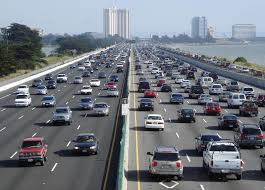
\includegraphics[width=0.5\textwidth]{traffic_scene}
    \caption{Typical High-Way Traffic Scene}
    \label{fig:hh_traffic}
  \end{center}
\end{figure}

The scenes also have varying light according to the time of the day, and proposed solutions need to adapt to these changes as fast as possible, otherwise data might be lost. Other weather conditions can also interfere with the analysis, such as fog and rain, and need to be addressed when designing solutions.

\subsection{Our Challenge}

The "Analytics Server" module of the "Video Server" project had a list of requirements that needed to be \todo{Acabar}

Detetar eventos relevantes
	Contra mao
	Objetos caidos

Contar Veiculos

Apenas para camaras fixas


\section{Foreground Segmentation}

Image segmentation is the process through which  an image is separated into its different regions according to the desired output, usually objects of interest. These regions are composed by pixels that have a common characteristic ~\cite{shapiro_computer_2001} dependant on the desired result. There are several ways one can accomplish an adequate segmentation of an image, and the most relevant ones to our purpose are described below.

\subsection{Background Subtraction}

Background Subtraction is a segmentation technique based on the analysis of the difference of consecutive frames and use that information to create a background model, a representation of what the image looks like without any moving objects present. Given the nature of the process, cameras must be static and although some research has been made to overcome this issue ~\cite{li_detection_2012} ~\cite{sheikh_background_2009} ~\cite{zamalieva_background_2014}, this is beyond the scope of the project, due to the requirements given.

There are however a number of different ways to implement the background subtraction developed across the years with increasing segmentation accuracy and computational performance. Piccardi presented an overview of the most relevant ones in ~\cite{piccardi_background_2004}, aiming to present each method's strengths and weaknesses. From this work we can present a list of the algorithms considered for implementation in the project.

\subsubsection{Frame Differencing}

This is the simplest approach to the problem as it only considers two frames at a time, making it only work in certain scenarios where the speed of the objects and frame rate of the camera allow it. In this model a pixel is considered as foreground if it satisfies the equation presented in ~\ref{eq:frame_diff}, and since the only parametrizable value is the Threshold, the whole segmentation process is very sensitive to any changes in this value.

\begin{eqnarray}
\label{eq:frame_diff}
\left | frame_{i} - frame_{i-1} \right | >= Threshold
\end{eqnarray}
\subsubsection{History Based Background Model}

In order to make this segmentation method more robust, in the early 2000's Velastin ~\cite{lo_automatic_2001} and Cucchiara ~\cite{cucchiara_detecting_2003} proposed a mathematical model to take into consideration past frames when calculating the Background Model of the scene. The most simple version of the improved algorithm used a running average of the past frames as seen in ~\ref{eq:running_average}. This eliminates the need to store the frames in memory as the new average can be calculated using the previous results.

\begin{eqnarray}
\label{eq:running_average}
BackgroundModel _{i+1} = \alpha * Frame_{i} + (1-\alpha)* BackgroundModel _{i}
\end{eqnarray}

Instead of the running average one can use the median value of the last n frames, improving the method reaction to outlying values. In both however, the history can be just the n frames or a weighted average where recent frames have more weight. Both these methods cannot cope with intermittent changes on the background, such as moving leaves against a building facade, and to solve this problem a new approach was proposed, the Mixture of Gaussians which models each pixel according to a mixture of Gaussian distributions, usually 3 to 5, but in later research ~\cite{zivkovic_improved_2004} a method was developed to calculate the number of distributions needed on a per pixel basis.

\subsection{Object Based}

Object Based segmentation relies on the a priori knowledge of the geometry of the objects we want to extract from the image. It is mainly used in medical applications such as in ~\cite{snell_model-based_1993} where it is used to extract a model of the brain surface from MRI scans \todo{Acabar}

\section{Image Treatment}

This section will review some of the proposed methods to improve image quality before or during processing by removing noise, extracting unwanted features or enhancing relevant features for the processes involved.

\subsection{Blur}

In order to blur an image one needs to convolve it using a special kind of filter. The process of convolution in image processing consists in the application of a filter to every pixel of an image, returning a new image where each pixel is the result of the function to the pixel in the same position in the previous image. As we can see in ~\ref{fig:convolution} the application of a 3*3 mask, where all 9 values have the value 1/9, results in a image where each pixel value equals the mean of itself and surrounding neighbours in the original image.

\begin{figure}[h]
  \begin{center}
    \leavevmode
    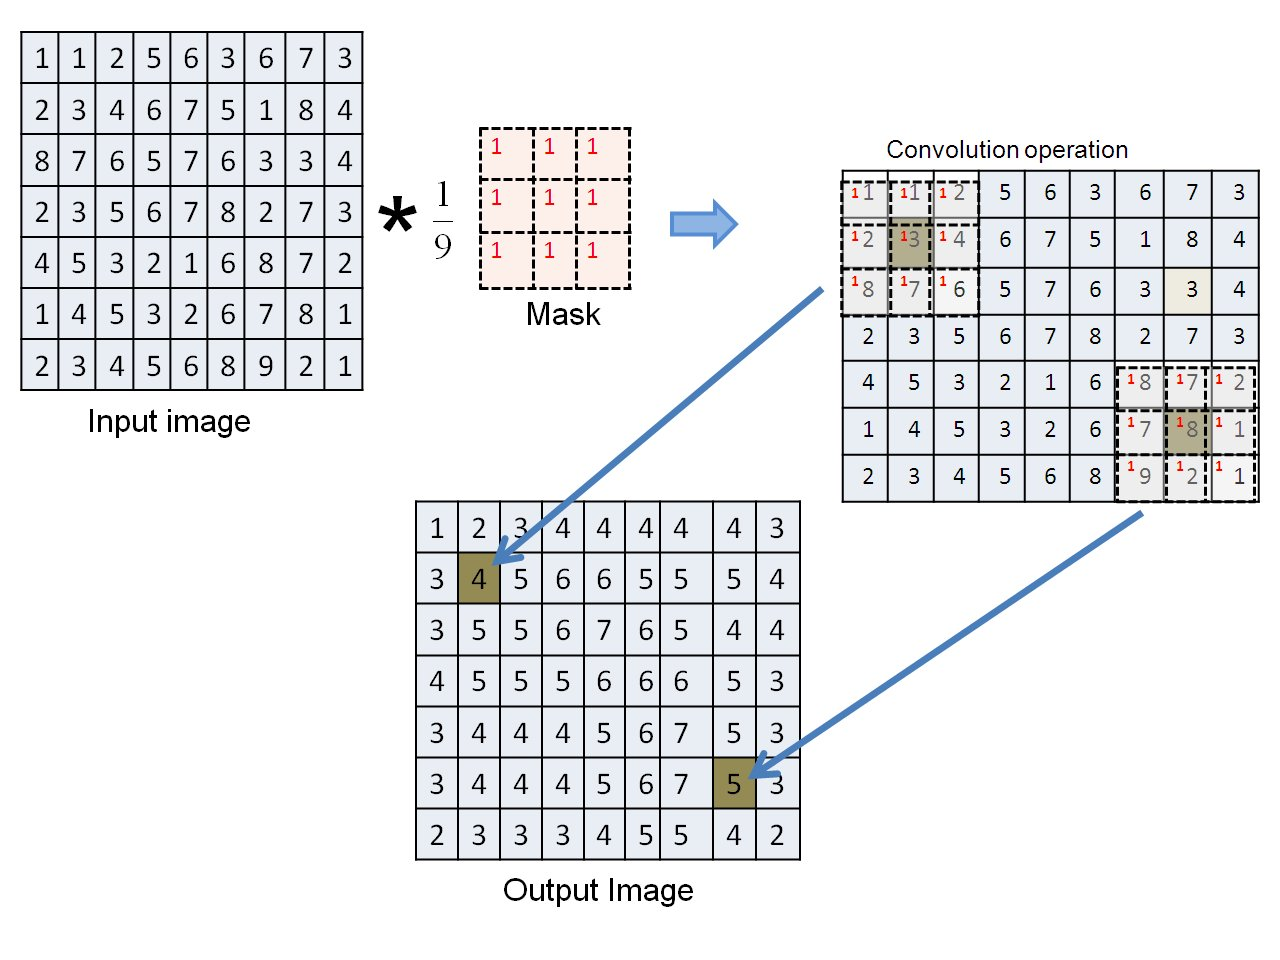
\includegraphics[width=0.5\textwidth]{convolution}
    \caption{Convolution Example (src: http://cse19-iiith.vlabs.ac.in/theory.php?exp=neigh)}
    \label{fig:convolution}
  \end{center}
\end{figure}
\todo{Verificar Imagem}

While this is the simplest blur processing we can apply to an image, there are more complex ones that yield better results. The one most often used in image processing is the Gaussian Blur, which uses a square filter with values calculated with the equation in ~\ref{eq:gaussian} from ~\cite{shapiro_computer_2001}.

\begin{eqnarray}
\label{eq:gaussian}
G(x,y) = \frac{1}{2\pi \sigma ^{2}}e^{-\frac{x^{2}+y^{2}}{2\sigma ^{2}}}
\end{eqnarray}

This equation returns a filter consisting of concentric circles that results in a smooth blurring of the images due to the application of the same power of blurring from equidistant pixels. The function can be tuned to the needs of the process through the $\sigma$ value, returning a sharper or softer blur filter as seen in ~\ref{fig:gaussian}.


\begin{figure}[h]
  \begin{center}
    \leavevmode
    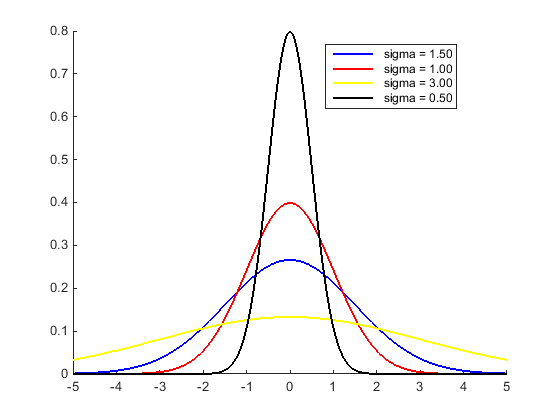
\includegraphics[width=0.5\textwidth]{gaussian}
    \caption{Gaussian Function Variation with Sigma Value}
    \label{fig:gaussian}
  \end{center}
\end{figure}

This kind of filters have multiple uses in computer vision

\subsection{Morphology Operators}

\subsection{Edge Detection}

\subsection{Shadow Removal}
Rain Removal
Shadow Removal

\section{Secção Exemplo}\label{sec:dialecto}

\emph{Scalable Vector Graphics}\index{SVG}\index{XML!SVG} é uma
linguagem em formato XML que descreve gráficos de duas dimensões. 
Este formato padronizado pela W3C (\emph{World Wide Web Consortium})
é livre de patentes ou direitos de autor e está totalmente
documentado, à semelhança de outros W3C
standards~cite{kn:svgdoc}.

Sendo uma linguagem XML, o \svg{} herda uma série de vantagens: a
possibilidade de transformar \svg{} usando técnicas como
XSLT\index{XML!XSLT}, de embeber \svg{} em qualquer documento
XML\index{XML} usando \textit{namespaces} ou até de  
estilizar \svg{} recorrendo a CSS\index{CSS} (\emph{Cascade Style Sheets}). 
De uma forma geral, pode dizer-se que \svg{}s interagem bem com as
atuais tecnologias ligadas ao XML e à Web, tal como referido
em~cite{kn:svgibm,kn:svgw3c}.

\section{Resumo ou Conclusões}

No final do capítulo deverá ser apresentado um resumo com as 
principais conclusões que se podem tirar. 

Vivamus non nunc nec risus tempor varius. Quisque bibendum mi at
dolor. Aliquam consectetuer condimentum risus. Aliquam luctus pulvinar
sem. Duis aliquam, urna et vulputate tristique, dui elit aliquet nibh,
vel dignissim magna turpis id sapien. Duis commodo sem id
quam. Phasellus dolor. Class aptent taciti sociosqu ad litora torquent
per conubia nostra, per inceptos himenaeos. 

\chapter{Visualização de Sinópticos SVG}\label{chap:chap3}

\section*{}

Este capítulo deve começar por fazer uma apresentação detalhada do
problema a resolver\footnote{Na introdução a apresentação do
  problema foi breve.} podendo mesmo, caso se justifique,
constituir-se um capítulo com essa finalidade.

Deve depois dedicar-se à apresentação da solução sem detalhes de
implementação. 
Dependendo do trabalho, pode ser uma descrição mais teórica, mais
``arquitetural'', etc.

\section{Secção Exemplo}

Neste capítulo apresentam-se exemplos de formatação de figuras e
tabelas, equações e referências cruzadas.

Apresenta-se de seguida um exemplo de equação, completamente fora do contexto:
\begin{eqnarray}
CIF_1: \hspace*{5mm}F_0^j(a) &=& \frac{1}{2\pi \iota} \oint_{\gamma} \frac{F_0^j(z)}{z - a} dz\\
CIF_2: \hspace*{5mm}F_1^j(a) &=& \frac{1}{2\pi \iota} \oint_{\gamma} \frac{F_0^j(x)}{x - a} dx \label{eq:cif}
\end{eqnarray}

Na Equação~\ref{eq:cif} lorem ipsum dolor sit amet, consectetuer
adipiscing elit. Suspendisse tincidunt viverra elit. Donec tempus
vulputate mauris. Donec arcu. Vestibulum condimentum porta
justo. Curabitur ornare tincidunt lacus. Curabitur ac massa vel ante
tincidunt placerat. Cras vehicula semper elit. Curabitur gravida, est
a elementum suscipit, est eros ullamcorper quam, sed cursus velit
velit tempor neque. Duis tempor condimentum ante.

Phasellus imperdiet, orci vel pretium sollicitudin, magna nunc
ullamcorper augue, non venenatis dui nunc quis massa. Pellentesque
dolor elit, dapibus venenatis, viverra ultricies, accumsan cursus,
orci. Aliquam erat volutpat. Mauris ornare tristique leo. Maecenas
eros. Curabitur velit nunc, tincidunt vitae, dictum posuere, pulvinar
nec, diam. In suscipit mauris a nunc. Pellentesque gravida. Morbi quam
lacus, pretium eget, tincidunt vulputate, interdum sed,
turpis. Curabitur quis est. Sed lectus lorem, congue vel, dignissim
laoreet, blandit a, nisi. Aenean nunc ligula, tincidunt eu, hendrerit
vel, suscipit non, erat. Aliquam gravida. Integer non pede. In laoreet
augue id leo. Mauris placerat. 

A arquitetura do visualizador assenta sobre os seguintes conceitos
basecite{kn:ZPMD97}: 

\begin{itemize}
\item \textbf{Componentes} --- Suspendisse auctor mattis augue \emph{push};
\item \textbf{Praesent} --- Sit amet sem maecenas eleifend facilisis leo;
\item \textbf{Pellentesque} --- Habitant morbi tristique senectus et netus.
\end{itemize}

\subsection{Exemplo de Figura}

É apresentado na Figura~\ref{fig:arch} %da página~\pageref{fig:arch}
um exemplo de figura flutuante.

\begin{figure}[t]
  \begin{center}
    \leavevmode
    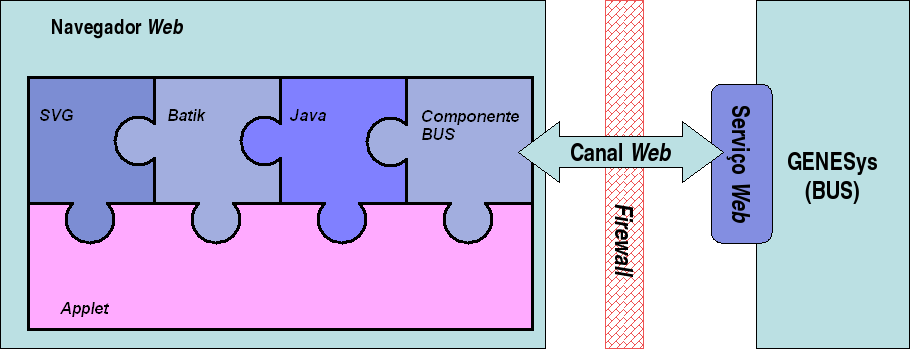
\includegraphics[width=0.86\textwidth]{puzzle}
    \caption{Arquitectura da Solução Proposta}
    \label{fig:arch}
  \end{center}
\end{figure}

Loren ipsum dolor sit amet, consectetuer adipiscing elit. 
Praesent sit amet sem. Maecenas eleifend facilisis leo. Vestibulum et
mi. Aliquam posuere, ante non tristique consectetuer, dui elit
scelerisque augue, eu vehicula nibh nisi ac est. Suspendisse elementum
sodales felis. Nullam laoreet fermentum urna. 

Duis eget diam. In est justo, tristique in, lacinia vel, feugiat eget,
quam. Pellentesque habitant morbi tristique senectus et netus et
malesuada fames ac turpis egestas. Fusce feugiat, elit ac placerat
fermentum, augue nisl ultricies eros, id fringilla enim sapien eu
felis. Vestibulum ante ipsum primis in faucibus orci luctus et
ultrices posuere cubilia Curae; Sed dolor mi, porttitor quis,
condimentum sed luctus. 

\subsection{Exemplo de Tabela}

É apresentado na Tabela~\ref{tab:exemplo1} um exemplo de tabela
flutuante e na Tabela~\ref{tab:exemplo2} um exemplo de tabela
flutuante, um pouco mais complicada.

\begin{table}[t]
  \centering
  \caption{Uma Tabela Simples}
\begin{tabular}{| l | p{45mm} |}
	\hline
\textbf{Acrónimo} & \textbf{Significado}\\
	\hline
	\hline
        ADT   & \emph{Abstract Data Type}\\\hline
        ANDF  & \emph{Architecture-Neutral Distribution Format}\\\hline
        API   & \emph{Application Programming Interface}\\
	\hline
\end{tabular}
  \label{tab:exemplo1}
\end{table}

Integer quis pede. Fusce nibh. Fusce nec erat vel mi condimentum
convallis. Sed at tortor non mauris pretium aliquet. In in lacus in
dolor molestie dapibus. Suspendisse potenti. Pellentesque sagittis
porta erat. Mauris sodales sapien id augue. Nam eu dolor. Donec sit
amet turpis non orci rhoncus commodo. Etiam condimentum commodo
libero.

Mauris pede. Curabitur faucibus dictum nibh. Proin tincidunt diam
vitae mauris. Sed hendrerit dolor vel ipsum. Nullam dapibus. Vivamus
tellus diam, egestas sit amet, vulputate non, vulputate id, eros. Nunc
sit amet nibh eget nibh imperdiet ornare. Cras vehicula mattis
ipsum. Sed diam arcu, semper at, gravida vitae, fermentum et,
nulla. Aenean massa orci, tristique nec, rutrum id, fringilla eget,
erat. Curabitur nulla ipsum, aliquam sed, rutrum vitae, semper quis,
ante. Fusce at nunc in dolor condimentum tempor. Duis sit amet massa. 

Curabitur convallis nulla quis risus. Nulla mollis porttitor
purus. Fusce ultricies odio at ligula pellentesque suscipit. Nulla
velit libero, blandit a, aliquet quis, hendrerit id, arcu. Phasellus
porttitor porttitor purus. Suspendisse velit tortor, fringilla sit
amet, commodo a, ultrices et, mi. Donec eu metus in erat ornare
adipiscing. Praesent varius mi ac nunc. Vestibulum leo lacus,
elementum in, vestibulum sit amet, hendrerit at, justo. Sed sit amet
neque. Donec libero risus, commodo sit amet, dignissim ut, tincidunt
a, eros. Ut non lacus quis tortor mattis ullamcorper. Vivamus
consequat augue vel erat. Sed tincidunt. Sed leo eros, ornare a,
pulvinar non, mattis quis, nibh. Aliquam faucibus mi ac nisi.

Pellentesque habitant morbi tristique senectus et netus et malesuada
fames ac turpis egestas. Duis aliquet, libero sit amet ornare viverra,
augue erat interdum dolor, vitae tincidunt lorem erat a lacus. Sed
lectus nisi, auctor in, hendrerit a, molestie vel, lectus. Cum sociis
natoque penatibus et magnis dis parturient montes, nascetur ridiculus
mus. Duis lacinia tempor dui. Vivamus rhoncus, tellus a viverra
dignissim, pede dui adipiscing odio, non faucibus metus mi gravida
eros. Nullam a tellus ut velit elementum tempus. Aenean rutrum
convallis tellus. Vestibulum nulla ante, dapibus ut, lobortis ut,
varius sed, nisl. Fusce lobortis. Sed ac lorem. Nulla tincidunt nulla
eget leo. Maecenas ac lectus eu neque ultrices pharetra. Curabitur a
risus nec arcu placerat tempor. Suspendisse magna nisl, viverra a,
adipiscing eget, ornare ultricies, ligula. Maecenas eu ligula vitae
eros convallis dignissim. 

\begin{table}[t]
  \centering
  \caption{Uma Tabela Mais Complicada}
\begin{tabular}{|c|r@{.}lr@{.}lr@{.}l||r|}
	\hline
\multicolumn{8}{|c|}
	{\rule[-3mm]{0mm}{8mm}Iteração $k$ de $f(x_n)$} \\
\textbf{\em k}
	& \multicolumn{2}{c}{$x_1^k$}
	& \multicolumn{2}{c}{$x_2^k$}
	& \multicolumn{2}{c||}{$x_3^k$}
	& comentários \\ \hline \hline
0   & -0&3                 & 0&6                 &  0&7   & - \\
1   &  0&47102965 & 0&04883157 & -0&53345964  & $\delta<\epsilon$ \\
2   &  0&49988691 & 0&00228830 & -0&52246185  & $\delta < \varepsilon$ \\
3   &  0&49999976 & 0&00005380 & -0&523656   &   $N$ \\
4   &  0&5                 & 0&00000307 & -0&52359743  & \\
\vdots	& \multicolumn{2}{c}{\vdots}
	& \multicolumn{2}{c}{$\ddots$}
	& \multicolumn{2}{c||}{\vdots}  & \\
7   &  0&5   & 0&0    & \textbf{-0}&\textbf{52359878}
		 & $\delta<10^{-8}$ \\ \hline
\end{tabular}
  \label{tab:exemplo2}
\end{table}

Loren ipsum dolor sit amet, consectetuer adipiscing elit. 
Praesent sit amet sem. Maecenas eleifend facilisis leo. Vestibulum et
mi. Aliquam posuere, ante non tristique consectetuer, dui elit
scelerisque augue, eu vehicula nibh nisi ac est. Suspendisse elementum
sodales felis. Nullam laoreet fermentum urna. 

Duis eget diam. In est justo, tristique in, lacinia vel, feugiat eget,
quam. Pellentesque habitant morbi tristique senectus et netus et
malesuada fames ac turpis egestas. Fusce feugiat, elit ac placerat
fermentum, augue nisl ultricies eros, id fringilla enim sapien eu
felis. Vestibulum ante ipsum primis in faucibus orci luctus et
ultrices posuere cubilia Curae; Sed dolor mi, porttitor quis,
condimentum sed luctus. 

\section{Secção Exemplo}

Loren ipsum dolor sit amet, consectetuer adipiscing elit. 
Praesent sit amet sem. Maecenas eleifend facilisis leo. Vestibulum et
mi. Aliquam posuere, ante non tristique consectetuer, dui elit
scelerisque augue, eu vehicula nibh nisi ac est. Suspendisse elementum
sodales felis. Nullam laoreet fermentum urna. 

Duis eget diam. In est justo, tristique in, lacinia vel, feugiat eget,
quam. Pellentesque habitant morbi tristique senectus et netus et
malesuada fames ac turpis egestas. Fusce feugiat, elit ac placerat
fermentum, augue nisl ultricies eros, id fringilla enim sapien eu
felis. Vestibulum ante ipsum primis in faucibus orci luctus et
ultrices posuere cubilia Curae; Sed dolor mi, porttitor quis,
condimentum sed luctus. 

\section{Resumo e Conclusões}

Resumir e apresentar as conclusões que se podem tirar no fim deste
capítulo.

%!TEX root = mieic-en.tex

\chapter{Implementation}\label{chap:chap4}
\listoftodos
\section*{}

\textit{
Este capítulo pode ser dedicado à apresentação de detalhes de nível
mais baixo relacionados com o enquadramento e implementação das
soluções preconizadas no capítulo anterior.
Note-se no entanto que detalhes desnecessários à compreensão do
trabalho devem ser remetidos para anexos.
Dependendo do volume, a avaliação do trabalho pode ser incluída neste
capítulo ou pode constituir um capítulo separado.
}


As previously stated, the work done for this project consists of a module for the "Video Server" being developed by LIACC, that will perform all the required analytics of the video received. This chapter provides the details of the implementation of this module, developed during the dissertation semester between February and June 2017. Tasks performed involved designing an appropriate architecture, able to scale with the project, treating the images received from the video streams to detect events and extract information. 

It is expected that this chapter provides some insight on how the theoretical backgrounds presented before were used during the project development, namely phase 2 and 3 of the presented project planning\missingfigure{Project Planning}. Phase 2 focused on the detection of relevant events to the traffic controller such as suspicious approximation to the camera, intrusion in prohibited areas, fallen objects on the road and wrong way travelling, while phase 3 aimed to count and classify vehicles in both urban and high-way scenarios.

\section{Technology}

In order to build this project we needed both a library of already implemented computer vision algorithms as well as a simple way to retrieve frames from both video streams and files. This section describes what were the chosen technologies including a brief description and why it was chosen.

\subsection{OpenCV}
OpenCV is a library composed of implementations of useful computer vision algorithms implementation, widely used across the industry and academy. It has interfaces for multiple programming languages, like C++, Java and Python, but is natively written in C++ in order to take advantage of low level performance enhancements, as performance is an important factor in real time computer vision applications.

The library contains over 2500 algorithms ranging from the more basic image processing such as filtering, morphology operators and geometric transformations to more complex ones that are able to, among others, compare images, track features and camera movements and recognize faces. Along with the image processing capabilities OpenCV also ships with interfaces to stereo cameras such as Kinect that allow users to retrieve a cloud of 3D points and a depth map from the captured image. This was the chosen library as there existed already previous work at LIACC using it, which could be leveraged for this project.

\subsection{JavaCV}
JavaCV is a wrapper for OpenCV written in Java that works on top of the JavaCPP Presets, a project that provides Java interfaces for commonly used C++ libraries, such as OpenCV and FFmpeg\todo{Adicionar referencias}, the ones we are using, as well as CUDA, ARToolKitPlus and others. It provides access to all the functionalities of OpenCV inside a Java environment, and was the chosen solution as there was already experience inside LIACC working with this technology.

\subsection{FFmpeg}
FFmpeg is a framework that performs encoding, decoding, transcoding, streaming and filter operations on videos in all the well known video formats, across a large number of platforms. It is used in the "Video Server" to read streams from any format and restream them all to the same format. In the Analytic module it is used to grab the frames from both the video files and the streams using the same methods.

\begin{lstlisting}[float,language=Java, label=src:ffmpegframegrabber, caption=FFmpegFrameGrabber usage example] 
// videopath can be either a stream path or a file path
FFmpegFrameGrabber _frameGrabber = FFmpegFrameGrabber.createDefault(videopath);
Frame currentFrame = null;

while( (currentFrame = _frameGrabber.grabImage()) != null) {
	// Use grabbed frame
}
\end{lstlisting}

\section{Architecture}

\subsection{Implementation Architecture}

\missingfigure{Diagrama Arquitetura}

The analytics module was designed to comply with the following specifications, imposed by both our partner and to comply with the already developed modules. 

\begin{itemize}
	\item Run uninterruptedly waiting for requests to be made
	\item Process a large number of video inputs at the same time
	\item Receive input from streams or files
	\item Specify which analysis are to be run on a specific video
\end{itemize}
\todo{Mais requirements?}

The project main thread runs an instance of the AnalyticsManager class that implements the Java Runnable interface. This thread will launch one CameraAnalyticsManager instance for each video to be analysed, be it from stream or from file, and keep track of each worker status, disposing of them when they finish, and launching new ones when a request is received. The CameraAnalyticsManager is then responsible to query the database in order to find out what are the analytics the user wants to retrieve from the video, information that is stored in the \textit{camera} table of the database. This process then starts a frame grabber that will convert each frame of the video into its representation in OpenCV and feed it to each Analyser through a queue. This enables each one of these workers to run at his own pace and if one of them runs slower than the pace at which the frame grabber reads the images, it will simply queue them up and not slow down the remaining workers. The drawbacks of this solution are that it is theoretically possible to run out of memory to keep these frames, although this limit was not reached during the testing phase.

\subsection{Database}

\todo{Sera relevante?}
Camaras sao o principal ator

Videos (streams e ficheiros) estao associados a uma camara


\section{Segmentation}

This section describes how the segmentation of the received images is performed, and how it returns a foreground mask representing the moving areas of the scene, specifying through what processors and filters it is passed through. \todo{Overview do processo?}

\begin{figure}[t]
  \begin{center}
    \leavevmode
    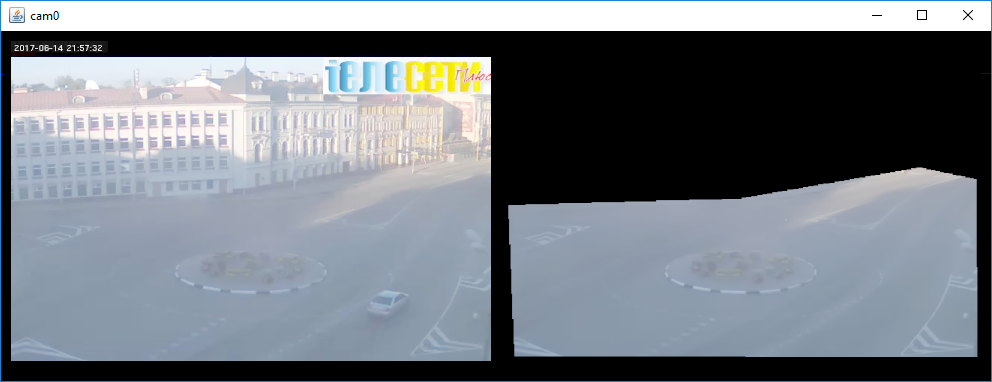
\includegraphics[width=0.95\textwidth]{bgsub_01}
    \caption{Background Subtraction - Background Model}
    \label{fig:bgsub_01}
  \end{center}
\end{figure}

In ~\ref{fig:bgsub_01} we can see the original frame on the left and the calculated background model of the scene on the right. To achieve this result, the first step is to mask the obtained frame \todo{Explain masking process} in order to prevent uninteresting regions of the image from being processed the Background Subtracter. This solves an issue where moving or changing regions of the image outside our region of interest would create unwanted artefacts, for example moving trees due to the wind blowing, or the issue that occurred in this scene, where a car passing would be reflected in the windows of the building.

The next step of the Segmentation process is to feed the masked frames into a Background Subtraction algorithm that will use them to update its internal representation of the scene. This project uses the OpenCV implementation of the Mixture of Gaussians algorithm that allows the user to tune:

\begin{itemize}
	\item Number of past frames considered on the background calculation
	\item Threshold value from which a pixel is considered to be foreground, compared to the difference between its current value and the one from the background model
	\item Learning rate of the algorithm, how much each new frame influences the model
\end{itemize}

After updating the background model we can retrieve from the Background Subtracter its foreground mask, a rough representation that is calculated by subtracting the background model from the current image and thresholding it, thus returning only the pixels where the difference is significant enough.

\begin{figure}[t]
  \begin{center}
    \leavevmode
    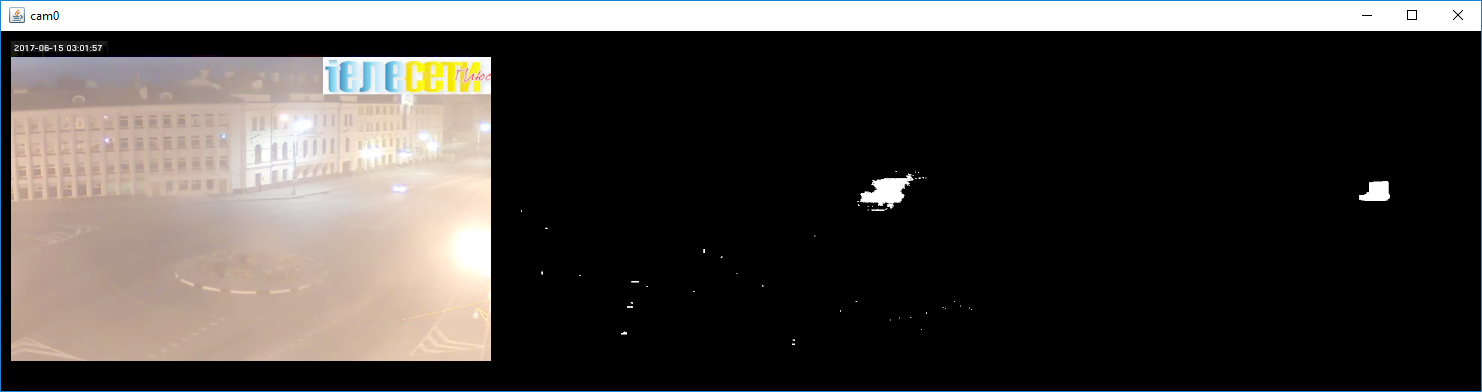
\includegraphics[width=0.95\textwidth]{bgsub_03}
    \caption{Background Subtraction - Foreground Mask}
    \label{fig:bgsub_02}
  \end{center}
\end{figure}

As we can see in the middle image of figure~\ref{fig:bgsub_02} the foreground mask from the Background Subtracter can have a lot of noise due to lighting conditions. To solve this issue two morphology filters are applied to the image, a squared erosion filter to remove the small speckles that appear in the mask, followed by a larger circular dilation filter to consolidate the positive regions of the mask, as the wind shield and windows of the vehicles are usually detected as background due to their dark colour and/or reflection of the environment.

\section{Object Detection}

When we have a foreground mask clean of noise and with solid regions we proceed to detect them and retrieve their position and size from the mask. \missingfigure{Deteçao dos Objetos}

OpenCV provides BlobDetector, a family of functions that retrieve information of blobs in an image. It works by thresholding the image into multiple binary images using a range of threshold values, grouping the connected white pixels at each one of these images in binary blobs and then merging blobs that are close enough to each other into larger blobs.

This however does not work as intended for our input, an already binarized image where we just need to group the connected pixels. For this the project uses the OpenCV function \textit{connectedComponentsWithStats}, that retrieves the groups of connected pixels in a binary image along with their area, width, height and both the leftmost and topmost coordinate of the group's bounding box. From this data we can create an ImageObject instance that will represent a moving object in the scene, using the regions with a region size above a given threshold, in order to prevent detection of small objects or noise that got through the filtering process.

\section{Object Tracking}
\missingfigure{Tracking dos Objetos}

In order for the solution to correctly analyse  the objects of the scene it needs to track them during their lifetime, in other words, establish a relation between the objects identified on a frame with the objects identified in the next frame.

This is done iterating through each one of the new objects and finding which existing object is closer to him. If the distance between them is smaller than the size of the existing object then they are matched. To enhance this mechanism a sub-set of the state machine presented \todo{Referenciar artigo da state machine} which allows us to model the life cycle of an object. 

% State machine


% Velocity prediction

\section{Utility}

\subsection{Video Wall}

\subsection{Image Processors}

\section{Secção Exemplo}

%\todofigure{Inserir uma figura sobre o Map/Reduce}

Lorem ipsum dolor sit amet, consectetuer adipiscing elit. Integer
hendrerit commodo ante. Pellentesque nibh libero, aliquam at, faucibus
id, commodo a, velit. 
%\todoline{Escrever sobre o map/reduce}
Duis eleifend sem eget leo. Morbi in est. Suspendisse magna sem,
varius nec, hendrerit non, tincidunt quis, quam. Aenean congue. 
%\todolines{A short entry in the list of todos}{A very long todonote
%  that certainly will fill more than a single line in the list of
%  todos. Just to make sure let's add some more text.} 
Vivamus vel est sit amet sem iaculis posuere. Cras mollis, enim vel
gravida aliquam, libero nunc ullamcorper dui, ullamcorper sodales
lectus nulla sed urna. Morbi aliquet porta risus. 
Proin vestibulum ligula a purus. Maecenas a nulla. 
Maecenas mattis est vitae neque auctor tempus. Etiam nulla dui,
mattis vitae, porttitor sed, aliquet ut, enim. Cras nisl magna,
aliquet et, laoreet at, gravida ac, neque. Sed id est. Nulla dapibus
dolor quis ipsum rhoncus cursus.

\section{Mais uma Secção}

Lorem ipsum dolor sit amet, consectetuer adipiscing elit. Quisque
purus sapien, interdum ut, vestibulum a, accumsan ullamcorper,
erat. Mauris a magna ut leo porta imperdiet. Donec dui odio, porta in,
pretium non, semper quis, orci. Quisque erat diam, pharetra vel,
laoreet ac, hendrerit vel, enim. Donec tristique luctus risus. Fusce
dolor est, eleifend id, elementum sit amet, varius vitae, neque. Morbi
at augue. Ut sem ligula, auctor vitae, facilisis id, pharetra non,
lectus. Nulla lacus augue, aliquam eget, sollicitudin sed, hendrerit
eu, leo. Suspendisse ac tortor. Mauris at odio. Etiam vehicula. Nam
lacinia purus at nibh. Aliquam fringilla lorem ac justo. Ut nec
enim. 
%\todoref{Citar Map/reduce}

Quisque ullamcorper. Aliquam vel magna. Sed pulvinar dictum
ligula. Sed ultrices dolor ut turpis. Vivamus sagittis orci malesuada
arcu venenatis auctor. Proin vehicula pharetra urna. Aliquam egestas
nunc quis nisl. Donec ullamcorper. Nulla purus. Ut suscipit lacus
vitae dui. Mauris semper. Ut eget sem. Integer orci. Nam vitae dui
eget nisi placerat convallis. 

\begin{lstlisting}[float,language=Java, label=src:mapreduce, caption=Example map and reduce functions for word counting]
map(String key, String value): 
// key: document name 
// value: document contents 
for each word w in value:
EmitIntermediate(w, "1");

reduce(String key, Iterator values):
// key: a word 
// values: a list of counts 
int result = 0;
for each v in values: 
result += ParseInt(v);

Emit(AsString(result))
\end{lstlisting}

Sed id lorem. Proin gravida bibendum lacus. Sed molestie, urna quis
euismod laoreet, diam dolor dictum diam, vitae consectetuer leo ipsum
id ante. Integer eu lectus non mauris pharetra viverra. In feugiat
libero ut massa. Morbi cursus, lorem sollicitudin blandit semper,
felis magna pellentesque lacus, ut rhoncus leo neque at tellus. Sed
mattis, diam eget eleifend tincidunt, ligula eros tincidunt diam,
vitae auctor turpis est vel nunc. In eu magna. Donec dolor metus,
egestas sit amet, ultrices in, faucibus sed, lectus. Etiam est enim,
vehicula pharetra, porta non, viverra vel, nunc. Ut non sem. Etiam nec
neque. 

\section{Resumo ou Conclusões}

Proin vehicula pharetra urna. Aliquam egestas
nunc quis nisl. Donec ullamcorper. Nulla purus. Ut suscipit lacus
vitae dui. Mauris semper. Ut eget sem. Integer orci. Nam vitae dui
eget nisi placerat convallis. 

%!TEX root = mieic-en.tex

\chapter{Conclusions and Future Work} \label{chap:concl}

\section*{}

This chapter presents an overview of the work done, as well as an evaluation of the state of completion achieved during the semester, followed by a list of the contributions and a foresight into the next steps of the project. 

\section{Contributions}

The contributions of the dissertation can by split into Technological, Scientific and Applicational contributions.

\textbf{Technological Contributions} During the dissertation work an issue was found when trying to process a frame in multiple threads at the same time. The solution first implemented meant that the frame collector had to wait for each thread to return for it to go fetch the next one, which meant that some of the threads could have potentially long waiting times. The solution now implemented, described in section ~\ref{sec:architecture}, creates a queue in each of the threads to where the frame collector sends the frames and from where the thread processing them reads them. This solution solves the waiting problem by making the threads totally independent from each other and ensures that the whole system performance is not capped if a slower thread is introduced.

\textbf{Scientific Contributions} One of the main contributions of the project is related to the tracking of stopped vehicles found in urban scenarios, as it was one of the gaps found during the literature review. To solve this issue an alteration is proposed in the segmentation process to keep track of the state of stopped vehicles. The first one is a stabilization step in the background subtraction initialization that waits for the background model to be steady. This steadiness is measured by the number of pixels updated in the last frame after the application of the background subtracter. This step ensures that the background is not initialized with stopped vehicles or other actors in the middle of the scene.

\textbf{Applicational Contributions} All the work developed was made taken into account that the application was to be used by our partners at Armis-Group for vehicle counting and classification in high-way scenarios and as such this was the main focus of the use-cases in which the project was tested. As of the writing of this document an application is being prepared to be tested at Infrastruturas de Portugal with more than 100 camera inputs.

\section{Objective Completion}

The work regarding this dissertation can be divided into two main objectives: event detection and vehicle counting. As specified in the beginning of chapter ~\ref{chap:chap4}, phase two of the project dealt with the event detection portion of the work and phase three with vehicle counting.

During the development of phase two the priority of features shifted to vehicle counting due to a commitment by our partner and as such this phase was aborted to begin the development of phase three. This meant that of the initial list of events to be detected: wrong way driving, suspicious camera approximation, prohibited zone entering and fallen objects only the first three were complete. Regarding phase three, all the points were implemented and the application is now able to successfully count and classify vehicles into the light and heavy categories.

\section{Publications}\label{sec:publications}
During the development of the project a paper was submitted to the "Artificial Transportation Systems and Simulation" workshop in the IEEE International Conference on Intelligent Transportation Systems 2017. The submitted paper is based on the work done during this presentation with emphasis on the ability to feed information onto traffic simulation systems, based on the data gathered from real world.

\section{Future Work}

During the dissertation work a number of challenges appeared that would be interesting to address.

\textbf{Solve the issue regarding object grouping} As of now the segmentation process cannot distinguish multiple objects occluded by one another or linked through a shadow, although there is written work about how to solve this. Implementing such a solution would improve the results of the counting process.

\textbf{Time counting} The counting process can accurately count vehicles but it cannot detect when a vehicle was counted. To do so in videos, a starting time would be required as well as the frame count and rate. In streams the application needs to take into account both the starting time and the stream delay.

\textbf{Intersection Analysis} It would be interesting to follow some of the work regarding intersection statistics and implement a module on top of the Analytics Module that would work specifically for such cases.
 

%%----------------------------------------
%% Final materials
%%----------------------------------------

%% Bibliography
%% Comment the next command if BibTeX file not used
%% bibliography is in ``myrefs.bib''
\PrintBib{myrefs}

%% comment next 2 commands if numbered appendices are not used
%%\appendix
%%\chapter{Loren Ipsum} \label{ap1:loren}

Depois das conclusões e antes das referências bibliográficas,
apresenta-se neste anexo numerado o texto usado para preencher a
dissertação.

\section{O que é o \emph{Loren Ipsum}?}

\emph{\textbf{Lorem Ipsum}} is simply dummy text of the printing and
typesetting industry. Lorem Ipsum has been the industry's standard
dummy text ever since the 1500s, when an unknown printer took a galley
of type and scrambled it to make a type specimen book. It has survived
not only five centuries, but also the leap into electronic
typesetting, remaining essentially unchanged. It was popularised in
the 1960s with the release of Letraset sheets containing Lorem Ipsum
passages, and more recently with desktop publishing software like
Aldus PageMaker including versions of Lorem Ipsum~\citep{kn:Lip08}. 

\section{De onde Vem o Loren?}

Contrary to popular belief, Lorem Ipsum is not simply random text. It
has roots in a piece of classical Latin literature from 45 BC, making
it over 2000 years old. Richard McClintock, a Latin professor at
Hampden-Sydney College in Virginia, looked up one of the more obscure
Latin words, consectetur, from a Lorem Ipsum passage, and going
through the cites of the word in classical literature, discovered the
undoubtable source. Lorem Ipsum comes from sections 1.10.32 and
1.10.33 of ``de Finibus Bonorum et Malorum'' (The Extremes of Good and
Evil) by Cicero, written in 45 BC. This book is a treatise on the
theory of ethics, very popular during the Renaissance. The first line
of Lorem Ipsum, ``Lorem ipsum dolor sit amet\ldots'', comes from a line in
section 1.10.32.

The standard chunk of Lorem Ipsum used since the 1500s is reproduced
below for those interested. Sections 1.10.32 and 1.10.33 from ``de
Finibus Bonorum et Malorum'' by Cicero are also reproduced in their
exact original form, accompanied by English versions from the 1914
translation by H. Rackham.

\section{Porque se usa o Loren?}

It is a long established fact that a reader will be distracted by the
readable content of a page when looking at its layout. The point of
using Lorem Ipsum is that it has a more-or-less normal distribution of
letters, as opposed to using ``Content here, content here'', making it
look like readable English. Many desktop publishing packages and web
page editors now use Lorem Ipsum as their default model text, and a
search for ``lorem ipsum'' will uncover many web sites still in their
infancy. Various versions have evolved over the years, sometimes by
accident, sometimes on purpose (injected humour and the like). 

\section{Onde se Podem Encontrar Exemplos?}

There are many variations of passages of Lorem Ipsum available, but
the majority have suffered alteration in some form, by injected
humour, or randomised words which don't look even slightly
believable. If you are going to use a passage of Lorem Ipsum, you need
to be sure there isn't anything embarrassing hidden in the middle of
text. All the Lorem Ipsum generators on the Internet tend to repeat
predefined chunks as necessary, making this the first true generator
on the Internet. It uses a dictionary of over 200 Latin words,
combined with a handful of model sentence structures, to generate
Lorem Ipsum which looks reasonable. The generated Lorem Ipsum is
therefore always free from repetition, injected humour, or
non-characteristic words etc. 


%% Index
%% Uncomment next command if index is required
%% don't forget to run ``makeindex mieic-en'' command
%\PrintIndex
\iffalse \bibliography{myrefs.bib} \fi
\end{document}
